%% ===========================================================================
%% Basic Matrix Multiplication in Different Languages -- class presentation
%% Beamer, 16:9, metropolis theme. 4 slides, about 4-5 minutes.
%% Compile from this folder:  pdflatex slides.tex
%% Figures are read from ../results/ (generated by plot_results.py).
%% ===========================================================================
\documentclass[aspectratio=169,11pt]{beamer}
\usetheme[progressbar=frametitle,sectionpage=none,numbering=fraction]{metropolis}

\usepackage[T1]{fontenc}
\usepackage[scaled=0.95]{helvet}
\usepackage{amsmath}
\usepackage{tikz}
\usetikzlibrary{arrows.meta,positioning,calc}
\graphicspath{{../results/}}
% \setbeameroption{show notes on second screen=right}   % uncomment to see speaker notes

%% ---- palette ----------------------------------------------------------------
%% C = navy, Java = purp, Python = brred (same hue families as the figures)
\definecolor{ink}{HTML}{1B1F24}
\definecolor{navy}{HTML}{0033A0}
\definecolor{brred}{HTML}{E3120B}
\definecolor{purp}{HTML}{9D00C9}
\definecolor{gold}{HTML}{F2A900}
\definecolor{muted}{HTML}{6B7280}
\definecolor{soft}{HTML}{F2F3F5}

\setbeamercolor{normal text}{fg=ink,bg=white}
\setbeamercolor{frametitle}{fg=white,bg=ink}
\setbeamercolor{progress bar}{fg=brred,bg=ink!25}
\setbeamercolor{title separator}{fg=brred}
\setbeamercolor{alerted text}{fg=brred}
\setbeamercolor{footline}{fg=muted}
\setbeamerfont{frametitle}{size=\Large,series=\bfseries}
\setbeamertemplate{itemize item}{\color{brred}\raisebox{0.15ex}{\scriptsize$\blacktriangleright$}}
\setbeamertemplate{itemize subitem}{\color{muted}\textendash}
\setlength{\leftmargini}{1.1em}

% TikZ styles with parameters must live outside frames
\tikzset{
  srcbox/.style={draw=#1,line width=0.9pt,rounded corners=2pt,fill=white,
                 font=\ttfamily\scriptsize,minimum width=2.25cm,minimum height=6.5mm},
  engine/.style={fill=#1,text=white,rounded corners=2pt,font=\scriptsize\bfseries,
                 minimum width=2.9cm,minimum height=6.5mm,align=center},
  result/.style={fill=soft,rounded corners=2pt,font=\scriptsize,
                 minimum width=2.5cm,minimum height=6.5mm,align=center},
  tag/.style={fill=#1!12,text=#1,rounded corners=3.2mm,font=\scriptsize\bfseries,
              minimum width=2.2cm,minimum height=6.5mm},
  flow/.style={-{Stealth[length=2mm]},thick,ink!45},
  badge/.style={fill=soft,rounded corners=3pt,minimum width=3.15cm,minimum height=1.15cm},
}

\newcommand{\muted}[1]{{\color{muted}#1}}
\newcommand{\bignum}[2]{{\color{brred}\fontsize{19}{21}\selectfont\bfseries #1}\\[-1pt]{\small #2}\par\vspace{5pt}}
\newcommand{\sdot}[1]{\tikz[baseline=-0.6ex]\fill[#1] (0,0) circle (3.2pt);}

\title{Execution Time \& Memory Scaling of Matrix Multiplication}
\subtitle{Comparing C, Java, and Python}
\author{Javier Ruano Hernández}
\institute{Big Data \,\textperiodcentered\, Assignment 1 \,\textperiodcentered\, ULPGC}
\date{October 2026}
% Title graphic: one row of A times one column of B gives one cell of C
\titlegraphic{\vspace*{-1.4em}\hfill
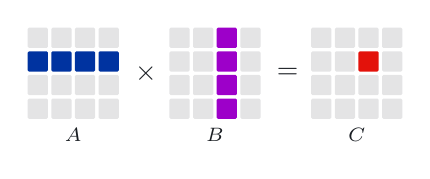
\begin{tikzpicture}[x=3.0mm,y=3.0mm]
  \foreach \r in {0,...,3} \foreach \c in {0,...,3} {
    % A: row 1 highlighted
    \ifnum\r=1 \def\fa{navy}\else\def\fa{ink!12}\fi
    \fill[\fa,rounded corners=0.5pt] (\c,-\r) rectangle ++(0.86,-0.86);
    % B: column 2 highlighted
    \ifnum\c=2 \def\fb{purp}\else\def\fb{ink!12}\fi
    \fill[\fb,rounded corners=0.5pt] (\c+6,-\r) rectangle ++(0.86,-0.86);
    % C: cell (1,2) highlighted
    \def\fcc{ink!12}
    \ifnum\r=1 \ifnum\c=2 \def\fcc{brred}\fi\fi
    \fill[\fcc,rounded corners=0.5pt] (\c+12,-\r) rectangle ++(0.86,-0.86);
  }
  \node[text=ink,font=\bfseries] at (5.0,-1.95) {$\times$};
  \node[text=ink,font=\bfseries] at (11.0,-1.95) {$=$};
  \foreach \x/\l in {1.93/A,7.93/B,13.93/C}
    \node[font=\scriptsize\bfseries,text=ink] at (\x,-4.55) {$\l$};
\end{tikzpicture}}

\begin{document}

%% ---------------------------------------------------------------------------
\maketitle
\note{(30 s) The same textbook triple loop, written in C, Java and Python. Question: how do runtime and memory grow
with the matrix size n, and how much does the execution model matter? Every element of C is a dot product of a row
of A and a column of B: 2n-cubed operations in total.}

%% ---------------------------------------------------------------------------
\begin{frame}{The Experiment}
\centering
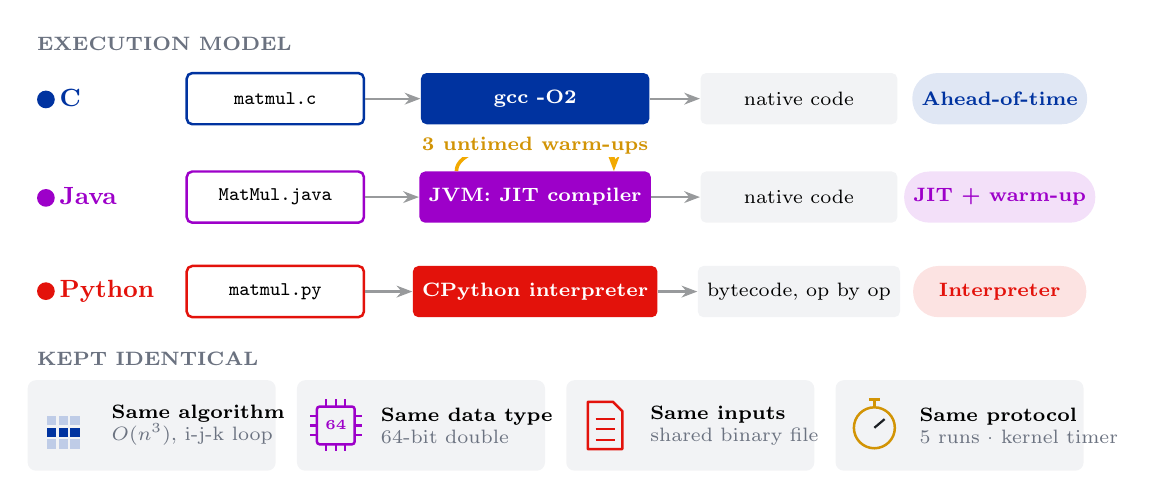
\begin{tikzpicture}
  % ---- three execution models ------------------------------------------------
  \node[anchor=west,font=\scriptsize\bfseries,text=muted] at (0,2.8) {EXECUTION MODEL};
  \foreach \y/\col/\lang/\src/\eng/\res/\tg in {
      2.1/navy/C/matmul.c/gcc -O2/{native code}/Ahead-of-time,
      0.85/purp/Java/MatMul.java/JVM: JIT compiler/{native code}/{JIT + warm-up},
     -0.35/brred/Python/matmul.py/CPython interpreter/{bytecode, op by op}/Interpreter} {
    \node[anchor=west,font=\small\bfseries,text=\col] at (0,\y) {\sdot{\col}\,\lang};
    \node[srcbox=\col] (s) at (3.15,\y) {\src};
    \node[engine=\col] (e) at (6.45,\y) {\eng};
    \node[result] (r) at (9.8,\y) {\res};
    \node[tag=\col] at (12.35,\y) {\tg};
    \draw[flow] (s) -- (e);
    \draw[flow] (e) -- (r);
  }
  % Java: untimed warm-up loop on the JIT
  \draw[-{Stealth[length=2mm]},gold,line width=1.3pt]
    (5.45,1.18) .. controls (5.45,1.66) and (7.45,1.66) .. (7.45,1.18);
  \node[font=\scriptsize\bfseries,text=gold!85!ink,fill=white,inner sep=1pt] at (6.45,1.5) {3 untimed warm-ups};

  % ---- controlled variables ------------------------------------------------------
  \node[anchor=west,font=\scriptsize\bfseries,text=muted] at (0,-1.2) {KEPT IDENTICAL};
  \foreach \x/\t/\s [count=\i] in {
      1.58/Same algorithm/{$O(n^3)$, i-j-k loop},
      5.0/Same data type/64-bit double,
      8.42/Same inputs/shared binary file,
      11.84/Same protocol/{5 runs \textperiodcentered\ kernel timer}} {
    \node[badge] (b\i) at (\x,-2.05) {};
    \node[anchor=west,align=left,font=\scriptsize] at ($(b\i.west)+(0.95,0)$)
      {\textbf{\t}\\\muted{\s}};
  }
  % icons
  \begin{scope}[shift={($(b1.west)+(0.25,-0.3)$)},x=1.5mm,y=1.5mm]   % grid = matrix
    \foreach \r in {0,1,2} \foreach \c in {0,1,2} {
      \ifnum\r=1 \def\ic{navy}\else\def\ic{navy!25}\fi
      \fill[\ic] (\c,\r) rectangle ++(0.82,0.82);}
  \end{scope}
  \begin{scope}[shift={($(b2.west)+(0.5,0)$)}]                      % chip = 64-bit
    \draw[purp,line width=0.9pt,rounded corners=1pt] (-0.24,-0.24) rectangle (0.24,0.24);
    \foreach \t in {-0.12,0,0.12} {
      \draw[purp,thick] (\t,0.24) -- (\t,0.33); \draw[purp,thick] (\t,-0.24) -- (\t,-0.33);
      \draw[purp,thick] (0.24,\t) -- (0.33,\t); \draw[purp,thick] (-0.24,\t) -- (-0.33,\t);}
    \node[font=\fontsize{5}{5}\selectfont\bfseries,text=purp] at (0,0) {64};
  \end{scope}
  \begin{scope}[shift={($(b3.west)+(0.5,0)$)}]                      % document = input file
    \draw[brred,line width=0.9pt,line join=round] (-0.22,-0.3) -- (-0.22,0.3) -- (0.1,0.3)
      -- (0.22,0.18) -- (0.22,-0.3) -- cycle;
    \foreach \t in {0.08,-0.05,-0.18} \draw[brred,thick] (-0.12,\t) -- (0.12,\t);
  \end{scope}
  \begin{scope}[shift={($(b4.west)+(0.5,-0.03)$)}]                  % stopwatch = timer
    \draw[gold!85!ink,line width=0.9pt] (0,0) circle (0.26);
    \draw[gold!85!ink,line width=0.9pt] (0,0.26) -- (0,0.34);
    \draw[gold!85!ink,thick] (-0.07,0.36) -- (0.07,0.36);
    \draw[ink,thick] (0,0) -- (0.13,0.11);
  \end{scope}
\end{tikzpicture}
\note{(1 min) Three ways of running the same loop. C is compiled ahead of time with gcc -O2. Java starts
interpreted and the JIT compiles the hot loop; three untimed warm-up runs let it reach full speed. Python executes
bytecode one operation at a time, with type checks and a heap object for every float. Everything else is held
constant: same algorithm and loop order, same 64-bit doubles, bit-identical inputs from one shared binary file,
five fresh-process runs, and only the kernel is timed. Results are checked against a correctly rounded reference
first.}
\end{frame}

%% ---------------------------------------------------------------------------
\begin{frame}{Empirical Scaling vs.\ Theoretical Model}
\begin{columns}[c]
\begin{column}{0.80\textwidth}
\centering
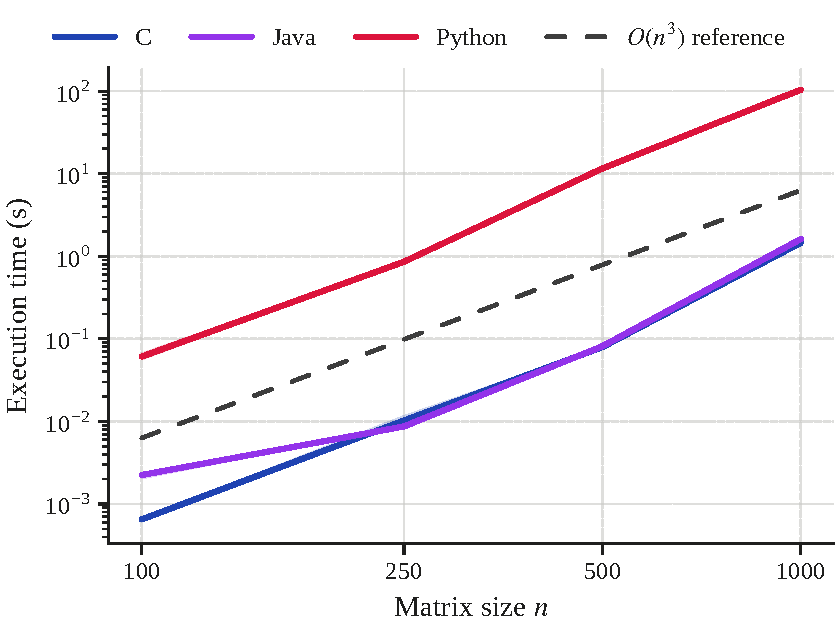
\includegraphics[width=0.495\linewidth]{time_vs_size}\hfill
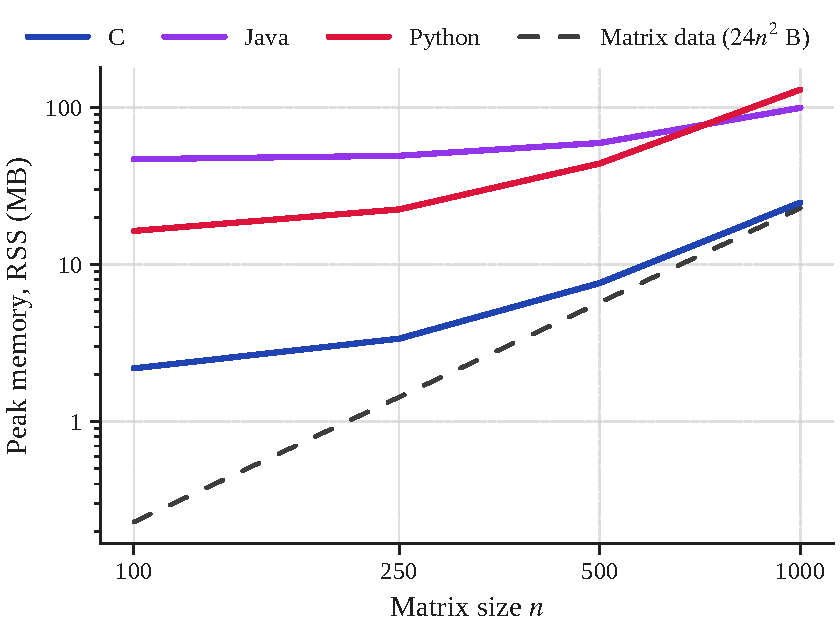
\includegraphics[width=0.495\linewidth]{memory_vs_size}\\[3pt]
{\scriptsize\muted{Median of 5 runs \textperiodcentered\ shaded: IQR \textperiodcentered\ log-log
\textperiodcentered\ dashed: $O(n^3)$ slope (left), $24n^2$ bytes of data (right)}}
\end{column}
\begin{column}{0.19\textwidth}
\bignum{3.3}{slope, C \& Python\\\muted{model: 3}}
\bignum{71{\boldmath$\times$}}{Python vs.\ C\\\muted{at $n=1000$}}
\bignum{47\,MB}{JVM baseline\\\muted{before any data}}
\end{column}
\end{columns}
\note{(1.5 min) Left: all three curves run roughly parallel to the n-cubed line, so the model predicts the trend.
But C and Java jump 18-20 times from 500 to 1000 instead of 8: a column of B no longer fits in the 48 KB L1 cache
and B approaches the 8 MB L3. Python hits the same limits one step earlier. Python is 71 to 146 times slower than C;
after warm-up, Java stays within 15 percent of C. Right: C sits almost on the data line, Java starts at about
47 MB for the JVM, and Python's boxed floats cost 5.7 times the data at n = 1000.}
\end{frame}

%% ---------------------------------------------------------------------------
\begin{frame}{Key Takeaways}
\centering
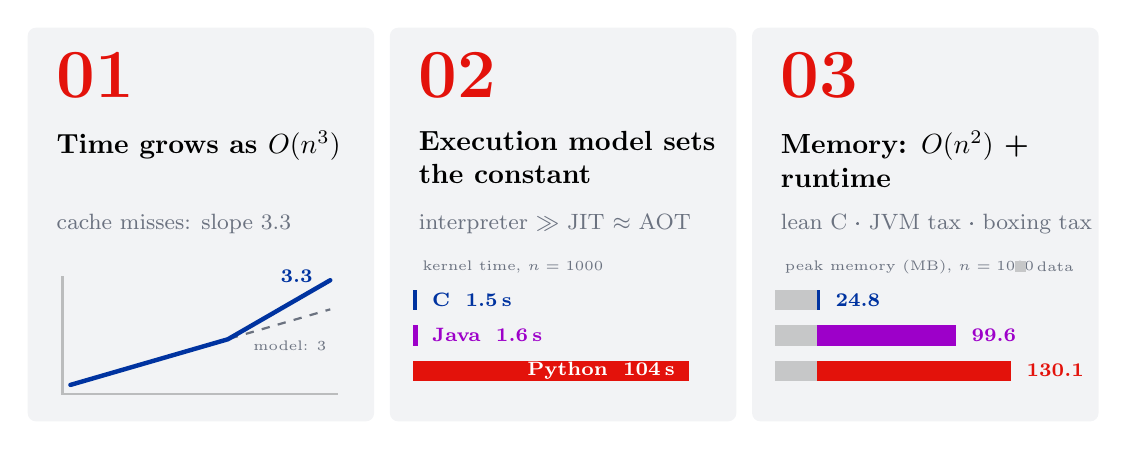
\begin{tikzpicture}[card/.style={rounded corners=3pt,fill=soft,minimum width=4.4cm,minimum height=5.0cm},
                    num/.style={anchor=north west,text=brred,font=\fontsize{26}{28}\selectfont\bfseries},
                    ttl/.style={anchor=north west,text width=3.95cm,align=flush left,font=\bfseries},
                    sub/.style={anchor=north west,text width=3.95cm,align=flush left,font=\footnotesize,text=muted},
                    hdr/.style={anchor=west,font=\tiny,text=muted}]
  \foreach \i in {1,2,3} \node[card] (c\i) at ({(\i-1)*4.6},0) {};

  % ---- 01: time ~ n^3 -----------------------------------------------------------
  \node[num] at ($(c1.north west)+(0.25,-0.2)$) {01};
  \node[ttl] at ($(c1.north west)+(0.25,-1.2)$) {Time grows as $O(n^3)$};
  \node[sub] at ($(c1.north west)+(0.25,-2.25)$) {cache misses: slope 3.3};
  \begin{scope}[shift={($(c1.south west)+(0.45,0.35)$)}]
    \draw[ink!30,thick] (0,1.5) -- (0,0) -- (3.5,0);
    \draw[muted,dashed,thick] (0.1,0.12) -- (3.4,1.08);
    \draw[navy,line width=1.6pt,line cap=round,line join=round] (0.1,0.12) -- (2.1,0.7) -- (3.4,1.45);
    \node[font=\tiny,text=muted,anchor=north west] at (2.3,0.8) {model: 3};
    \node[font=\scriptsize\bfseries,text=navy,anchor=east] at (3.3,1.5) {3.3};
  \end{scope}

  % ---- 02: execution model -------------------------------------------------------
  \node[num] at ($(c2.north west)+(0.25,-0.2)$) {02};
  \node[ttl] at ($(c2.north west)+(0.25,-1.2)$) {Execution model sets the constant};
  \node[sub] at ($(c2.north west)+(0.25,-2.25)$) {interpreter $\gg$ JIT $\approx$ AOT};
  \begin{scope}[shift={($(c2.south west)+(0.3,0.35)$)}]
    \node[hdr] at (0,1.62) {kernel time, $n=1000$};
    % bar lengths proportional to time: 103.8 s = 3.5 cm
    \fill[navy]  (0,1.07) rectangle ++(0.05,0.26);
    \fill[purp]  (0,0.62) rectangle ++(0.06,0.26);
    \fill[brred] (0,0.17) rectangle ++(3.5,0.26);
    \node[font=\scriptsize\bfseries,text=navy,anchor=west] at (0.12,1.2) {C \;1.5\,s};
    \node[font=\scriptsize\bfseries,text=purp,anchor=west] at (0.12,0.75) {Java \;1.6\,s};
    \node[font=\scriptsize\bfseries,text=white,anchor=east] at (3.45,0.3) {Python \;104\,s};
  \end{scope}

  % ---- 03: memory ----------------------------------------------------------------
  \node[num] at ($(c3.north west)+(0.25,-0.2)$) {03};
  \node[ttl] at ($(c3.north west)+(0.25,-1.2)$) {Memory: $O(n^2)$ + runtime};
  \node[sub] at ($(c3.north west)+(0.25,-2.25)$) {lean C \textperiodcentered\ JVM tax \textperiodcentered\ boxing tax};
  \begin{scope}[shift={($(c3.south west)+(0.3,0.35)$)}]
    \node[hdr] at (0,1.62) {peak memory (MB), $n=1000$};
    \fill[ink!25] (3.05,1.55) rectangle ++(0.14,0.14);
    \node[hdr] at (3.2,1.62) {data};
    % scale: 130 MB = 3.0 cm; grey = 22.9 MB of raw matrix data, colour = runtime overhead
    \foreach \y/\col/\w/\l in {1.2/navy/0.044/24.8, 0.75/purp/1.77/99.6, 0.3/brred/2.47/130.1} {
      \fill[ink!25] (0,\y-0.13) rectangle ++(0.53,0.26);
      \fill[\col] (0.53,\y-0.13) rectangle ++(\w,0.26);
      \node[font=\scriptsize\bfseries,text=\col,anchor=west] at (0.6+\w,\y) {\l};
    }
  \end{scope}
\end{tikzpicture}

\vspace{2mm}
{\scriptsize\muted{Scope: one machine (Ryzen AI 5 330, WSL 2) and one configuration \textemdash\ not a universal ranking}}
\note{(1 min) Three takeaways. One: time grows roughly as n cubed, but cache misses make the measured slope steeper
for C and Python. Two: the execution model sets the constant factor; the interpreter is 71 times slower than C,
while the JIT gets within 15 percent of ahead-of-time code. Three: memory is n squared plus a runtime cost: C needs
little more than the data, the JVM adds a fixed tax, and Python pays for every boxed float. All of this is for one
machine and configuration.}
\end{frame}

\end{document}
